\section{Математическая модель манипулятора}\label{part_math_model_of_robot}

\subsection{Кинематика манипулятора}\label{part_kinematics}

\subsubsection{Общие замечания}

% TODO Тут обосновать зачем нужна кинематика манипулятора

Последовательная кинематическая цепь рассматриваемого манипулятора, включающая только вращательные КП V-класса (цилиндрические шарниры), изображена на рисунке~\ref{img:kinematics}a.

\begin{figure}[h!]
	\begin{minipage}[h]{0.5\linewidth}
		\centering{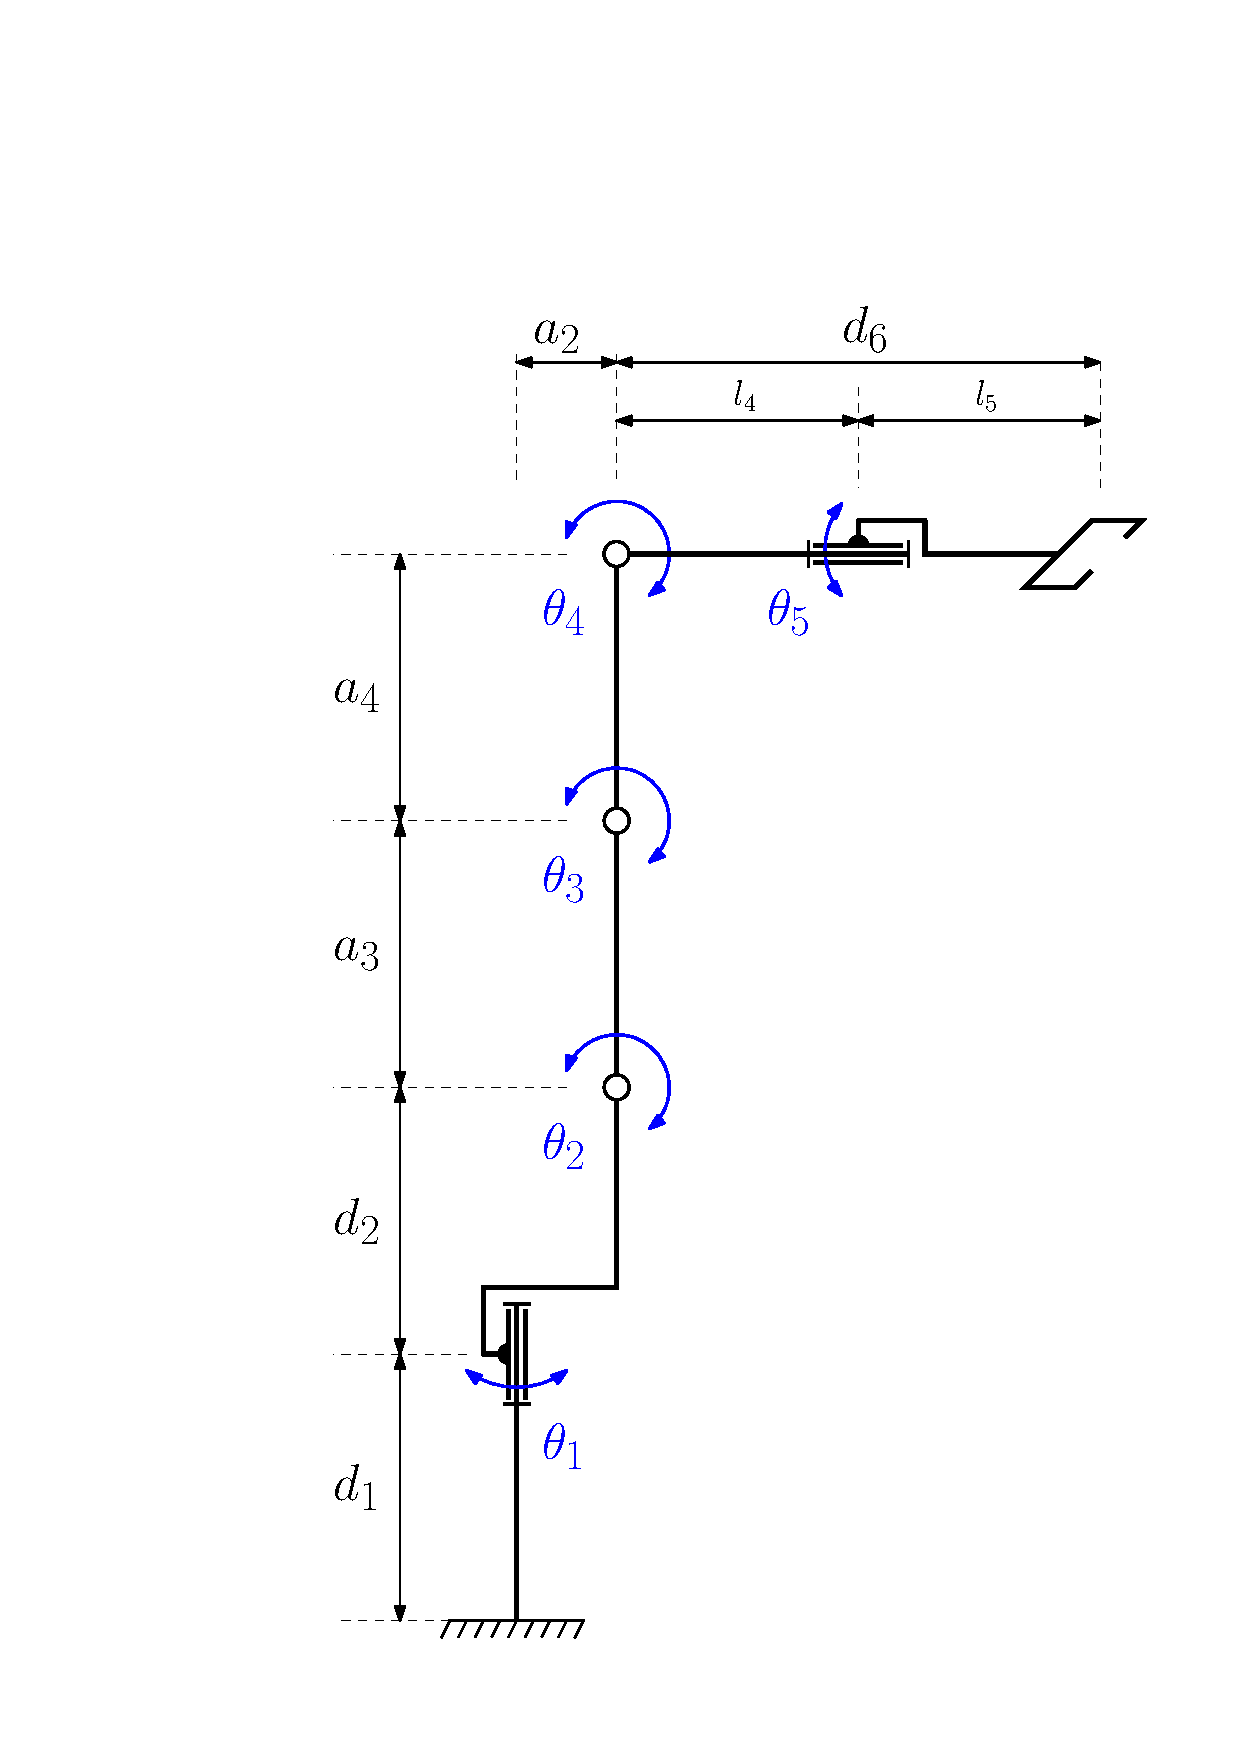
\includegraphics[width=0.95\linewidth]{kinematics_schema.pdf} \\ а)}
	\end{minipage}
	\hfill
	\begin{minipage}[h]{0.5\linewidth}
		\centering{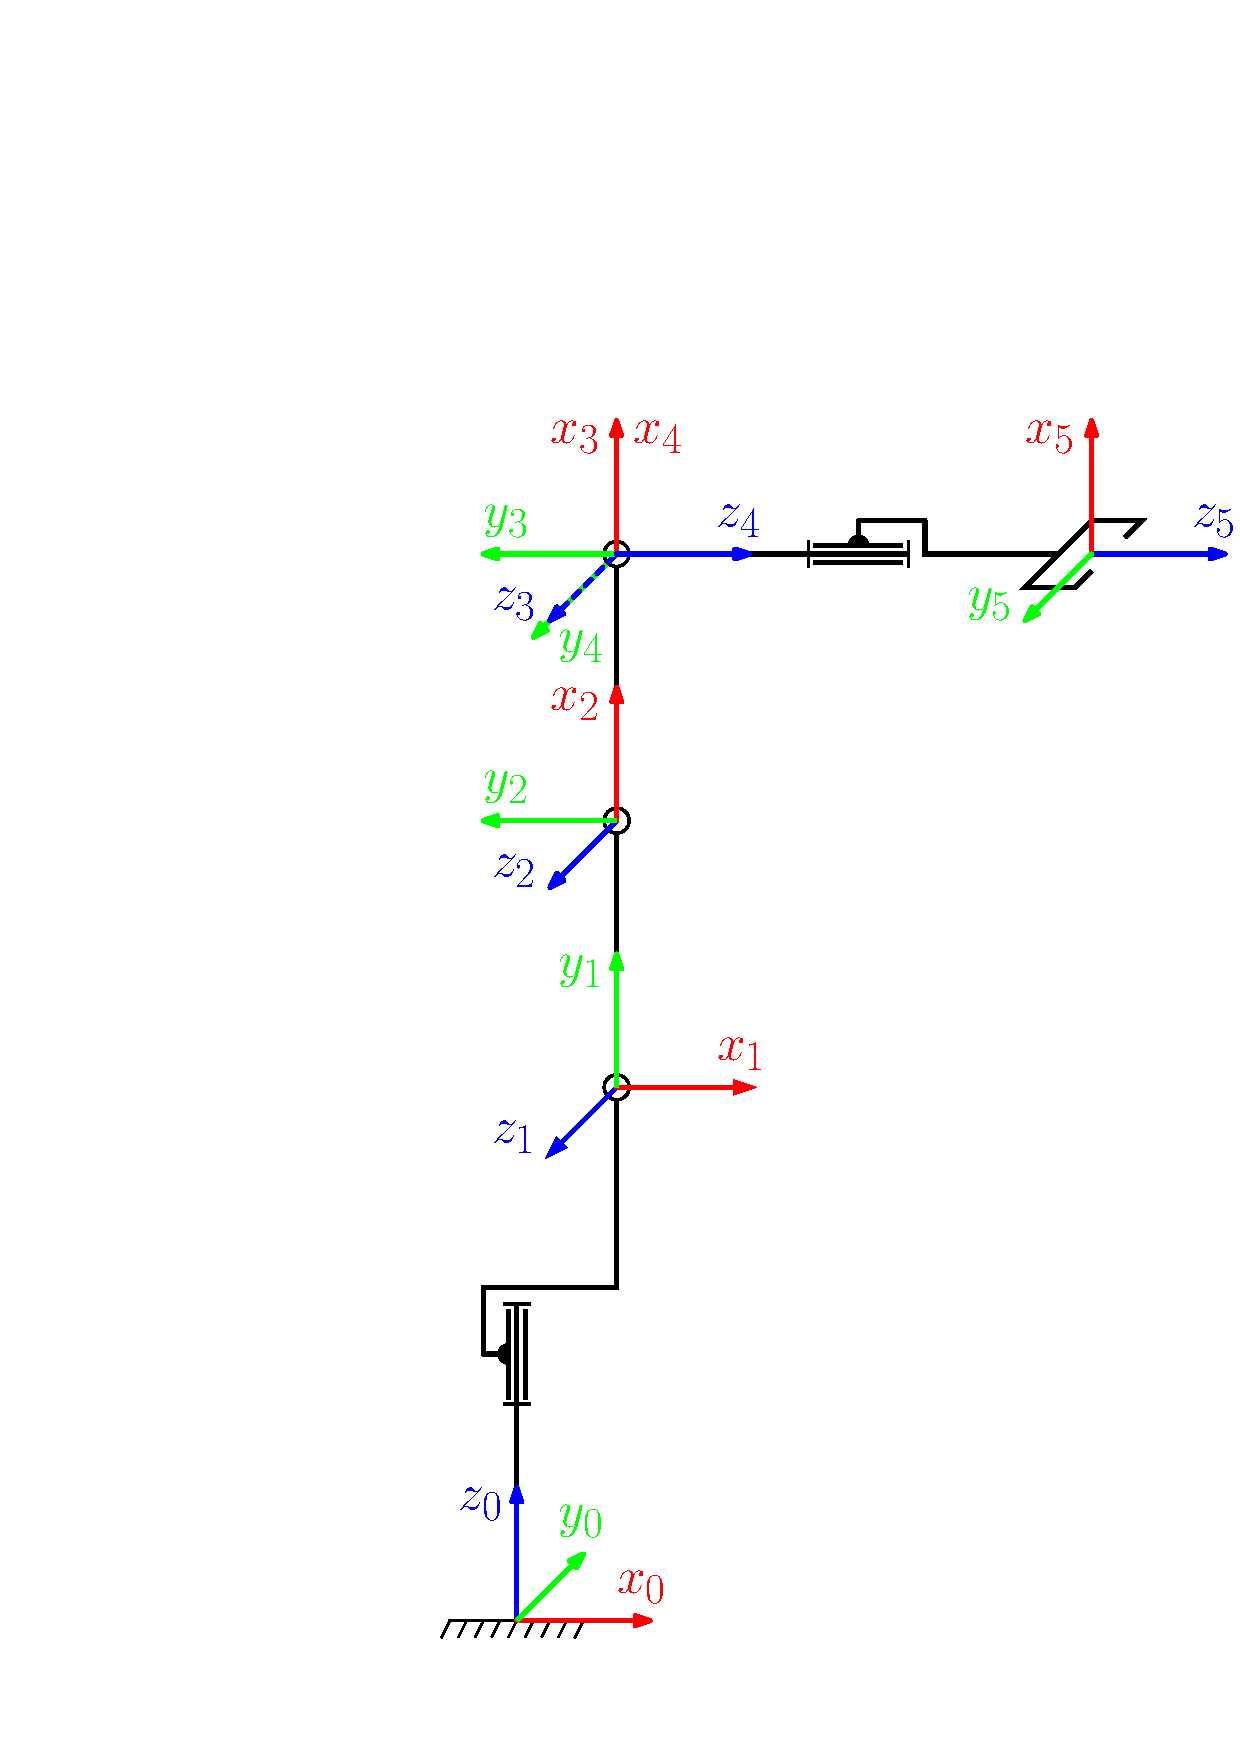
\includegraphics[width=0.95\linewidth]{kinematics_frames.pdf} \\ б)}
	\end{minipage}
	\caption{Схемы рассматриваемого манипулятора: а~--- кинематическая при $q_i=0$, $i=\overline{1,5}$; б~--- расположения СК КП.}
	\label{img:kinematics}
\end{figure}

Для описания положений звеньев манипулятора друг относительно друга воспользуемся методом Денавита--Хартенберга, состоящим из трех данных шагов:
\begin{enumerate}
    \item <<привязка>> к каждому звену СК, чьи оси удовлетворяют следующим условиям:
    \begin{enumerate}
	    \item ось $z_{i-1}$ направлена вдоль оси $i$-ой КП;
        \item ось $x_i$ перпендикулярна оси $z_{i-1}$ и пересекает ее;
        \item ось $y_i$ дополняет оси $z_i$ и $x_i$ до правой декартовой СК.
    \end{enumerate}
    \item определение параметров ДХ:
    \begin{enumerate}
	    \item $a_i$~--- расстояния от $z_{i-1}$ до $z_i$ вдоль $x_i$;
	    \item $\alpha_i$~--- угла от $z_{i-1}$ до $z_i$ вокруг $x_i$;
        \item $d_i$~--- расстояния от $x_{i-1}$ до $x_i$ вдоль $z_{i-1}$;
        \item $\theta_i$~--- угла от $x_{i-1}$ до $x_i$ вокруг $z_{i-1}$.
    \end{enumerate}
    \item расчет однородных матриц преобразования\footnote{За пояснениями обратитесь к Приложению~\ref{app_ht_matrices}} в соответствии со следующими формулами:
    \begin{equation}\label{DH_matrix}
        {}^{i-1}A_{i} = R_{z, \theta_i} \cdot T_{z, d_i} \cdot T_{x, a_i} \cdot R_{x, \alpha_i}
    \end{equation}
    где $R_{z, \theta_i}$~--- матрица поворота вокруг оси $z$ на угол $\theta_i$, $T_{z, d_i}$~--- матрица смещения вдоль оси $z$ на расстояние $d$, $T_{x, a_i}$~---матрица смещения вдоль оси $x$ на расстояние $a_i$,  $R_{x, \alpha_i}$~--- матрица поворота вокруг оси $x$ на угол $\alpha_i$, равные
    \begin{gather}
        R_{z, \theta_i} =
        \begin{bmatrix}
            \cos\theta_i & -\sin\theta_i & 0 & 0\\
            \sin\theta_i &  \cos\theta_i & 0 & 0\\
            0 & 0 & 1 & 0\\
            0 & 0 & 0 & 1
        \end{bmatrix}\!\!,
        \quad
        T_{z, d_i} =
        \begin{bmatrix}
            1 & 0 & 0 & 0\\
            0 & 1 & 0 & 0\\
            0 & 0 & 1 & d_i\\
            0 & 0 & 0 & 1\\
        \end{bmatrix}\!\!,\\
        %
        T_{x, a_i} =
        \begin{bmatrix}
            1 & 0 & 0 & a_i\\
            0 & 1 & 0 & 0\\
            0 & 0 & 1 & 0\\
            0 & 0 & 0 & 1\\
        \end{bmatrix}\!\!,
        \quad
        R_{x, \alpha_i} =
        \begin{bmatrix}
            1 & 0 & 0 & 0\\
            0 & \cos\alpha_i & -\sin\alpha_i & 0\\
            0 & \sin\alpha_i &  \cos\alpha_i & 0\\
            0 & 0 & 0 & 1
        \end{bmatrix}\!\!;
    \end{gather}
    итого
    \begin{equation}
        {}^{i-1}A_i =
        \begin{bmatrix}
            \cos\theta_i & - \cos\alpha_i \sin\theta_i & \sin\alpha_i \sin\theta_i & a_{i} \cos\theta_i\\
            \sin\theta_i & \cos\alpha_i \cos\theta_i & - \sin\alpha_i \cos\theta_i & a_{i} \sin\theta_i\\
            0 & \sin\alpha_i & \cos\alpha_i & d_{i}\\
            0 & 0 & 0 & 1
        \end{bmatrix}
    \end{equation}
\end{enumerate}

Результаты выполнения для исследуемого манипулятора двух первых шагов представлены на рисунке~\ref{img:kinematics}б и в таблице~\ref{table_DH_params}, а третьего~--- в лице следующих выражений:
\begin{gather}
	{}^0A_1\! =\!\!
    \left[\begin{matrix}c_{\theta_1} & 0 & s_{\theta_1} & a_{1} c_{\theta_1}\\s_{\theta_1} & 0 & - c_{\theta_1} & a_{1} s_{\theta_1}\\0 & 1 & 0 & d_{1}\\0 & 0 & 0 & 1\end{matrix}\right]\!\!;
    %
	{}^1A_2\! =\!\!
	\left[\begin{matrix}c_{\theta_2} & - s_{\theta_2} & 0 & a_{2} c_{\theta_2}\\s_{\theta_2} & c_{\theta_2} & 0 & a_{2} s_{\theta_2}\\0 & 0 & 1 & 0\\0 & 0 & 0 & 1\end{matrix}\right]\!\!;
    %
	{}^2A_3\! =\!\!
	\left[\begin{matrix}c_{\theta_3} & - s_{\theta_3} & 0 & a_{3} c_{\theta_3}\\s_{\theta_3} & c_{\theta_3} & 0 & a_{3} s_{\theta_3}\\0 & 0 & 1 & 0\\0 & 0 & 0 & 1\end{matrix}\right]\!\!;\notag
	\\
	{}^3A_4 =
	 \left[\begin{matrix}c_{\theta_4} & 0 & s_{\theta_4} & 0\\s_{\theta_4} & 0 & - c_{\theta_4} & 0\\0 & 1 & 0 & 0\\0 & 0 & 0 & 1\end{matrix}\right]\!\!;
	\;
	{}^4A_5 =
	\left[\begin{matrix}c_{\theta_5} & - s_{\theta_5} & 0 & 0\\s_{\theta_5} & c_{\theta_5} & 0 & 0\\0 & 0 & 1 & d_{5}\\0 & 0 & 0 & 1\end{matrix}\right]\!\!\ldotp
	\label{eq_all_ht_matrices}
\end{gather}

\begin{table}[h!]
	\caption{Параметры Денавита-Хартенберга}
	\begin{center}
		\begin{tabular}{|c|c|c|c|c|}
			\hline
			Звено 	& $a_i$, мм & $\alpha_i$, рад & $d_i$, мм & $\theta_i$, рад\\
			\hline
			1  		& $33$ & $\pi/2$ & $147$ & $q_1$\\
			\hline	
			2 		& $155$ & $0$ 	& $0$ 	& $q_2 + \pi/2$\\
			\hline
			3 		& $135$ & $0$ 	& $0$ 	& $q_3$\\
			\hline
			4 		& $0$ & $\pi/2$ & $0$ 	& $q_4$\\
			\hline
			5 		& $0$ & $0$ 	& $218$ & $q_5$\\
			\hline
		\end{tabular}
	\end{center}
	\label{table_DH_params}
\end{table}


\subsubsection{Прямая задача кинематики}\label{part_kinematics_forward}
Информация о смещении и повороте СК $Ox_5y_5z_5$ относительно СК $Ox_0y_0z_0$ содержится в матрице ${}^0A_5$.
Следовательно, для того чтобы решить ПЗК, остается лишь найти эту матрицу в соответствии c формулой:
\begin{equation}\label{fk}
	{}^0A_5 = \prod^{5}_{i=1}{{}^{i-1}A_i(q_i)}\ldotp
\end{equation}

\begin{figure}[h]
	\centering
	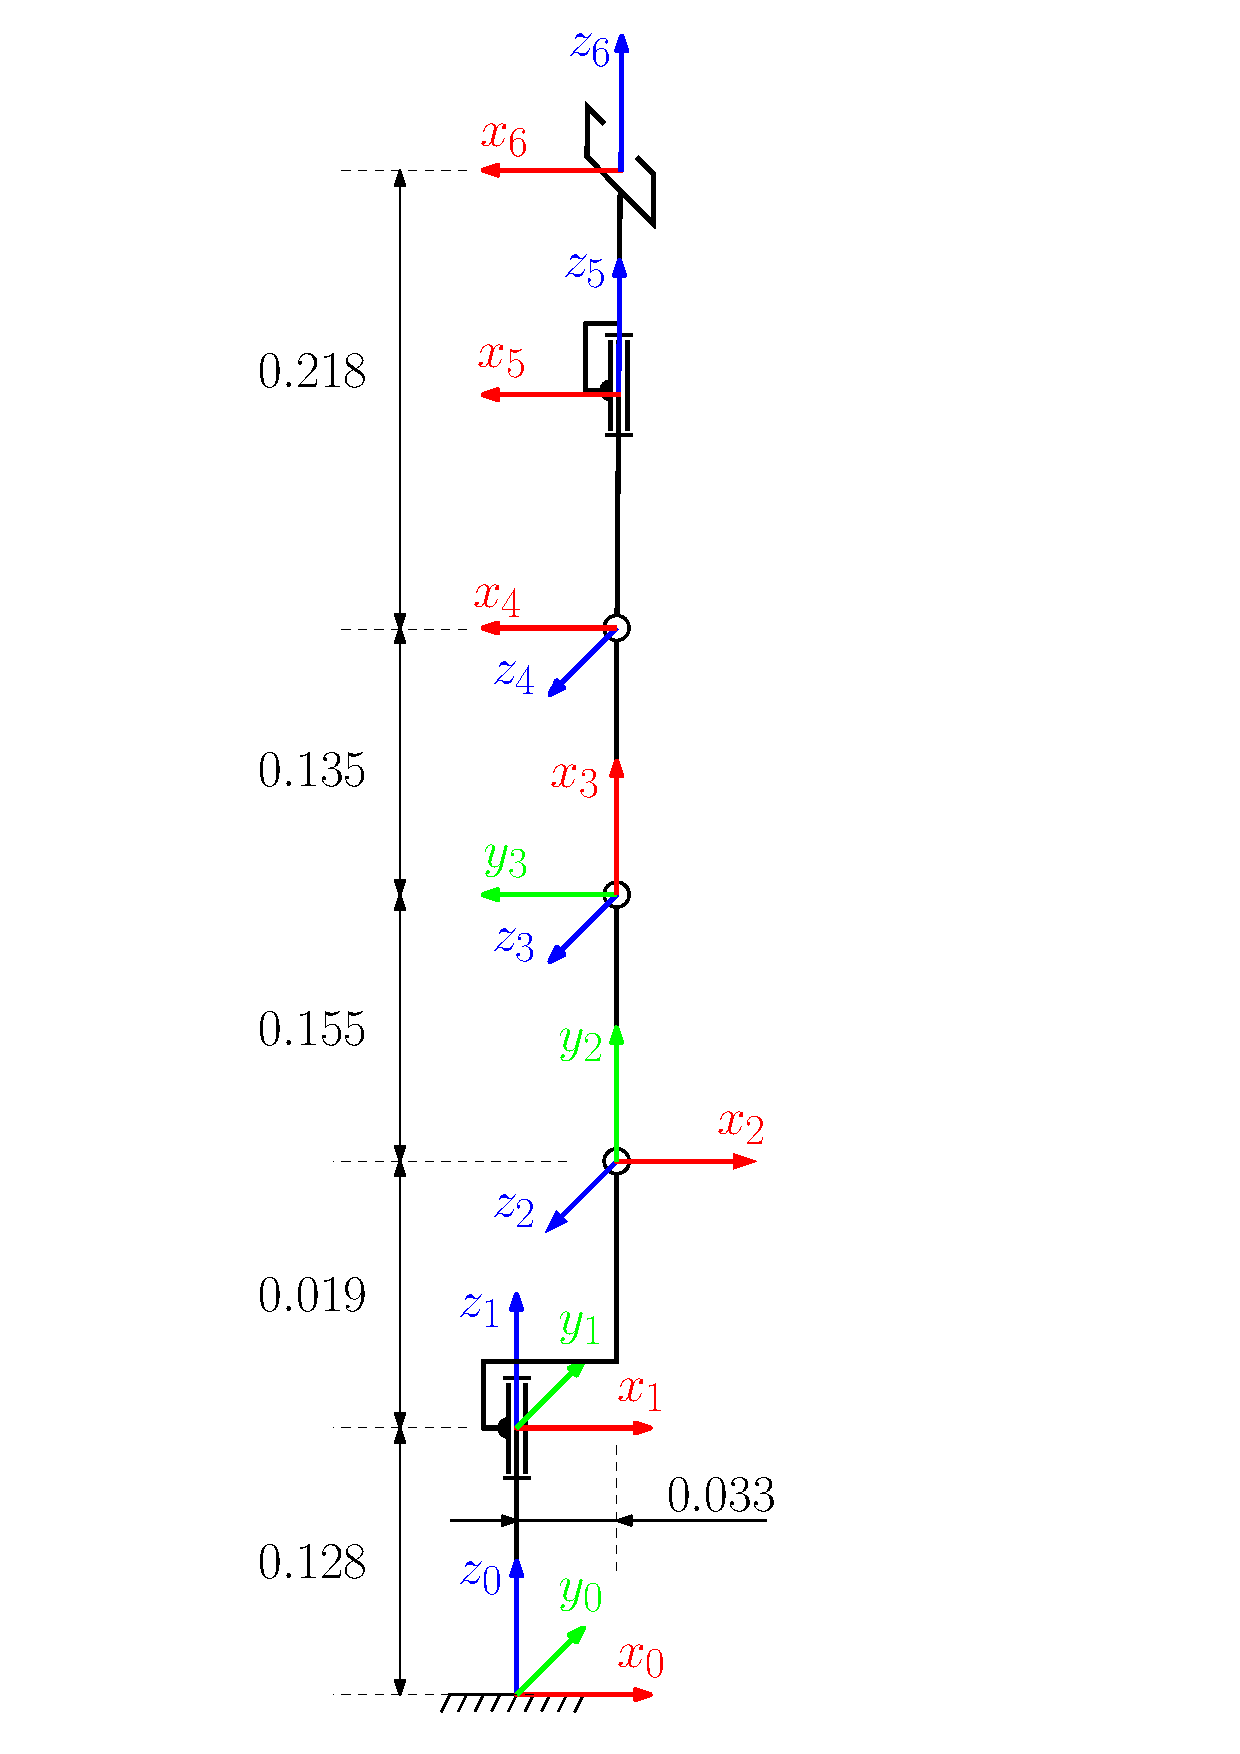
\includegraphics[width=0.2\textwidth]{kinematics_check.pdf}
	\caption{Конфигурация манипулятора при $q=\left[q_1,\,q_2,\,q_3,\,q_4,\,q_5\right] = \left[0,\,0,\,0,\,\pi/2,\,0\right]$.}
	\label{kinematics_check}
\end{figure}

Для проверки рассмотрим конфигурацию манипулятора, изображенную на рисунке~\ref{kinematics_check}.
В~результате решения для нее ПЗК должны получиться следующие матрица поворота и вектор смещения :
\begin{equation}
	{}^{0}R_5 =
	\begin{bmatrix}
		-1 &  0 & 0\\
		 0 & -1 & 0\\
		 0 &  0 & 1
	\end{bmatrix}\!\!,
	\qquad
	r^{0}_{0,\,5} =
	\begin{bmatrix}
		0.033\\
		0\\
		0.655 
	\end{bmatrix}\!\!\ldotp
\end{equation}
Выполняя соответствующие вычисления получаем:
\begin{multline}
    {}^{0}A_5 = {}^{0}A_1 \cdot {}^{1}A_2 \cdot {}^{2}A_3 \cdot {}^{3}A_4 \cdot {}^{4}A_5 =
    \begin{bmatrix}
        1 & 0 &  0 & 0.033\\
        0 & 0 & -1 &     0\\
        0 & 1 &  0 & 0.147\\
        0 & 0 &  0 &     1
    \end{bmatrix}
    \cdot
    \begin{bmatrix}
        0 & -1 &  0 &     0\\
        1 &  0 &  0 & 0.155\\
        0 &  0 &  1 &     0\\
        0 &  0 &  0 &     1
    \end{bmatrix}
    \cdot \\ \cdot
    \begin{bmatrix}
        1 & 0 &  0 & 0.135\\
        0 & 1 &  0 &     0\\
        0 & 0 &  1 &     0\\
        0 & 0 &  0 &     1
    \end{bmatrix}
    \cdot
    \begin{bmatrix}
        0 & 0 & 1 & 0\\
        1 & 0 & 0 & 0\\
        0 & 1 & 0 & 0\\
        0 & 0 & 0 & 1
    \end{bmatrix}
    \cdot
     \begin{bmatrix}
        1 & 0 &  0 &     0\\
        0 & 1 &  0 &     0\\
        0 & 0 &  1 & 0.218\\
        0 & 0 &  0 &     1
    \end{bmatrix}
    =
    \left[\begin{matrix}-1 & 0 & 0 & 0.033\\0 & -1 & 0 & 0\\0 & 0 & 1 & 0.655\\0 & 0 & 0 & 1\end{matrix}\right]\!\!,
\end{multline}
что предложенный способ решения ПЗК в данном случае приводит к правильному ответу.

\subsubsection{Обратная задача кинематики}\label{part_kinematics_inverse}
Заданные смещение и поворот СК $Ox_5y_5z_5$ относительно СК $Ox_0y_0z_0$ можно описать с помощью матрицы ${}^0A_5$.
Используя ее и матрицы из~\eqref{eq_all_ht_matrices}, найти расчетные формулы для углов $q_i$ ($i=\overline{1,5}$) можно из следующих соображений.

Введем обозначения для элементов матрицы ${}^0A_5$ в соответствии с формулой:
\begin{equation}\label{ik}
	{}^0A_5 =
	\left[\begin{matrix}
	r_{11} & r_{12} & r_{13} & p_{x}\\
	r_{21} & r_{22} & r_{23} & p_{y}\\
	r_{31} & r_{32} & r_{33} & p_{z}\\
	0 & 0 & 0 & 1
	\end{matrix}\right]\!\!\ldotp
\end{equation}

Приравняв матрицу ${}^0A_5$ и правую часть выражения~\eqref{fk} и домножив с обеих сторон на ${}^0A_1^{-1}$, придем к выражению:
\begin{equation}
	{}^0A_1^{-1} \cdot {}^0A_5 = {}^1A_2 \cdot {}^2A_3 \cdot {}^3A_4 \cdot {}^4A_5,
\end{equation}
где левая часть с учетом~\eqref{eq_all_ht_matrices} равна
\begin{equation}\label{eq_left_part}
	{}^0A_1^{-1} \cdot {}^0A_5 =
	\left[\begin{matrix}
		r_{11} c_{1} + r_{21} s_{1} & r_{12} c_{1} + r_{22} s_{1} & r_{13} c_{1} + r_{23} s_{1} &  p_{x} c_{1} + p_{y} s_{1} - a_{1}\\
		r_{31} & r_{32} & r_{33} & p_{z} - d_{1}\\
		r_{11} s_{1} - r_{21} c_{1} & r_{12} s_{1} - r_{22} c_{1} & r_{13} s_{1} - r_{23} c_{1} & p_{x} s_{1} - p_{y} c_{1}\\
		0 & 0 & 0 & 1\end{matrix}\right]\!\!,
\end{equation}
а правая~---
\begin{equation}\label{eq_right_part}
	{}^1A_2 \cdot {}^2A_3 \cdot {}^3A_4 \cdot {}^4A_5 =
	\left[\begin{matrix}
		c_{5} c_{234} & - s_{5} c_{234} & s_{234} & a_{2} c_{2} + a_{3} c_{23} + d_{5} s_{234}\\
		c_{5} s_{234} & - s_{5} s_{234} & - c_{234} & a_{2} s_{2} + a_{3} s_{23} - d_{5} c_{234}\\
		s_{5} & c_{5} & 0 & 0\\
		0 & 0 & 0 & 1
	\end{matrix}\right]\!\!,
\end{equation}
где в свою очередь
\begin{equation}\label{eq_theta_23_234}
    \theta_{23} = \theta_2 + \theta_3,
    \qquad
    \theta_{234} = \theta_2 + \theta_3 + \theta_4\ldotp
\end{equation}

Теперь, сопоставляя элементы матриц с одинаковыми индексами из выражений~\eqref{eq_left_part} и \eqref{eq_right_part}, получим, что расчетные формулы для двух наборов значений углов $\theta_1$, $\theta_5$ и $\theta_{234}$ дают
\begin{itemize}
    \item равенство элементов $(3,4)$:
        \begin{equation}\label{eq_for_theta_1}
	        p_{x} s_{1} - p_{y} c_{1} = 0
            \; \Rightarrow \;
	        \tg \theta_1 = \cfrac{p_y}{p_x}
	        \; \Rightarrow \;
	        \left\{
	        \begin{aligned}
		        \!&\theta_1^\msf{I} = \atan2(p_y, p_x)\\
		        \!&\theta_1^\msf{II} = \atan2(-p_y, -p_x)
            \end{aligned}
            \right.
        \end{equation}
    \item равенство элементов $(3,1)$ и $(3,2)$:
        \begin{multline}
            \left\{
	        \begin{aligned}
		        \!&s_{5} = r_{11} s_{1} - r_{21} c_{1}\\
		        \!&c_{5} = r_{12} s_{1} - r_{22} c_{1}
            \end{aligned}
            \right.
            \qquad \Rightarrow
            \\
            \Rightarrow \;
            \left\{
	        \begin{aligned}
		        \!&\theta_5^\msf{I} = \atan2(r_{11} \sin\theta_1^\msf{I} - r_{21} \cos\theta_1^\msf{I},\: r_{12} \sin\theta_1^\msf{I} - r_{22} \cos\theta_1^\msf{I})\\
		        \!&\theta_5^\msf{II} = \atan2(r_{11} \sin\theta_1^\msf{II} - r_{21} \cos\theta_1^\msf{II},\: r_{12} \sin\theta_1^\msf{II} - r_{22} \cos\theta_1^\msf{II})
            \end{aligned}
            \right.
        \end{multline}
    \item равенство элементов $(2,3)$ и $(1,3)$:
        \begin{multline}
            \left\{
	        \begin{aligned}
		        \!&c_{234} = -r_{33}\\
		        \!&s_{234} = r_{13} c_{1} + r_{23} s_{1}
            \end{aligned}
            \right.
            \qquad \Rightarrow
            \\
            \Rightarrow \qquad
            \left\{
	        \begin{aligned}
		        \!&\theta_{234}^\msf{I} = \atan2(r_{13} \cos\theta_1^\msf{I}  + r_{23} \sin\theta_1^\msf{I},\: -r_{33})\\
		        \!&\theta_{234}^\msf{II} = \atan2(r_{13} \cos\theta_1^\msf{II}  + r_{23} \sin\theta_1^\msf{II},\: -r_{33})
            \end{aligned}
            \right.
        \end{multline}
\end{itemize}

Далее домножим выражение~\eqref{eq_left_part} на ${}^4A_5^{-1}$ справа~--- получим матрицу~${}^1A_4$:
\begin{equation}\label{eq_A14_matrix}
    {}^1A_4 =
    \begin{bmatrix}
        \cdots & \cdots & \cdots & (p_y - d_5 r_{23})s_1 + (p_x - d_5 r_{13})c_1 - a_1\\
        \cdots & \cdots & \cdots & p_z - d_1 - d_5 r_{33}\\
        \cdots & \cdots & \cdots & p_x s_1 - p_y c_1 - d_5(r_{13} s_1 - r_{23} c_1)\\
        0 & 0 & 0 & 1
    \end{bmatrix}\!\!,
\end{equation}
в которой символами $\cdots$ обозначены элементы, не представляющие интереса в дальнейших расчетах.
Заметим, что c учетом~\eqref{eq_for_theta_1} и равенства элементов~$(3,3)$ в~\eqref{eq_left_part} и~\eqref{eq_right_part} справедливо
\begin{equation}
p_x s_1 - p_y c_1 - d_5(r_{13} s_1 - r_{23} c_1) = 0\ldotp
\end{equation}
С~учетом этого и~\eqref{eq_A14_matrix}, имеем что
\begin{equation}\label{eq_r_1_1_4}
    r^1_{1,\,4} =
    \begin{bmatrix}
        (p_y - d_5 r_{23})s_1 + (p_x - d_5 r_{13})c_1 - a_1 \\
        p_z - d_1 - d_5 r_{33} \\
        0
    \end{bmatrix}\!\!\ldotp
\end{equation}

Далее заметим, что одно и то же положение 4-го звена может достигаться при двух разных способах расположения звеньев~2 и~3 (см.~рисунок~\ref{ik_geometric}).
Следовательно, углы $\theta_2$, $\theta_3$ и $\theta_4$ при одних и тех же значениях углов $\theta_1$ и $\theta_5$ имеют по два возможных значения.
Ниже выводятся формулы для последних.

\begin{figure}[h!]
	\centering
	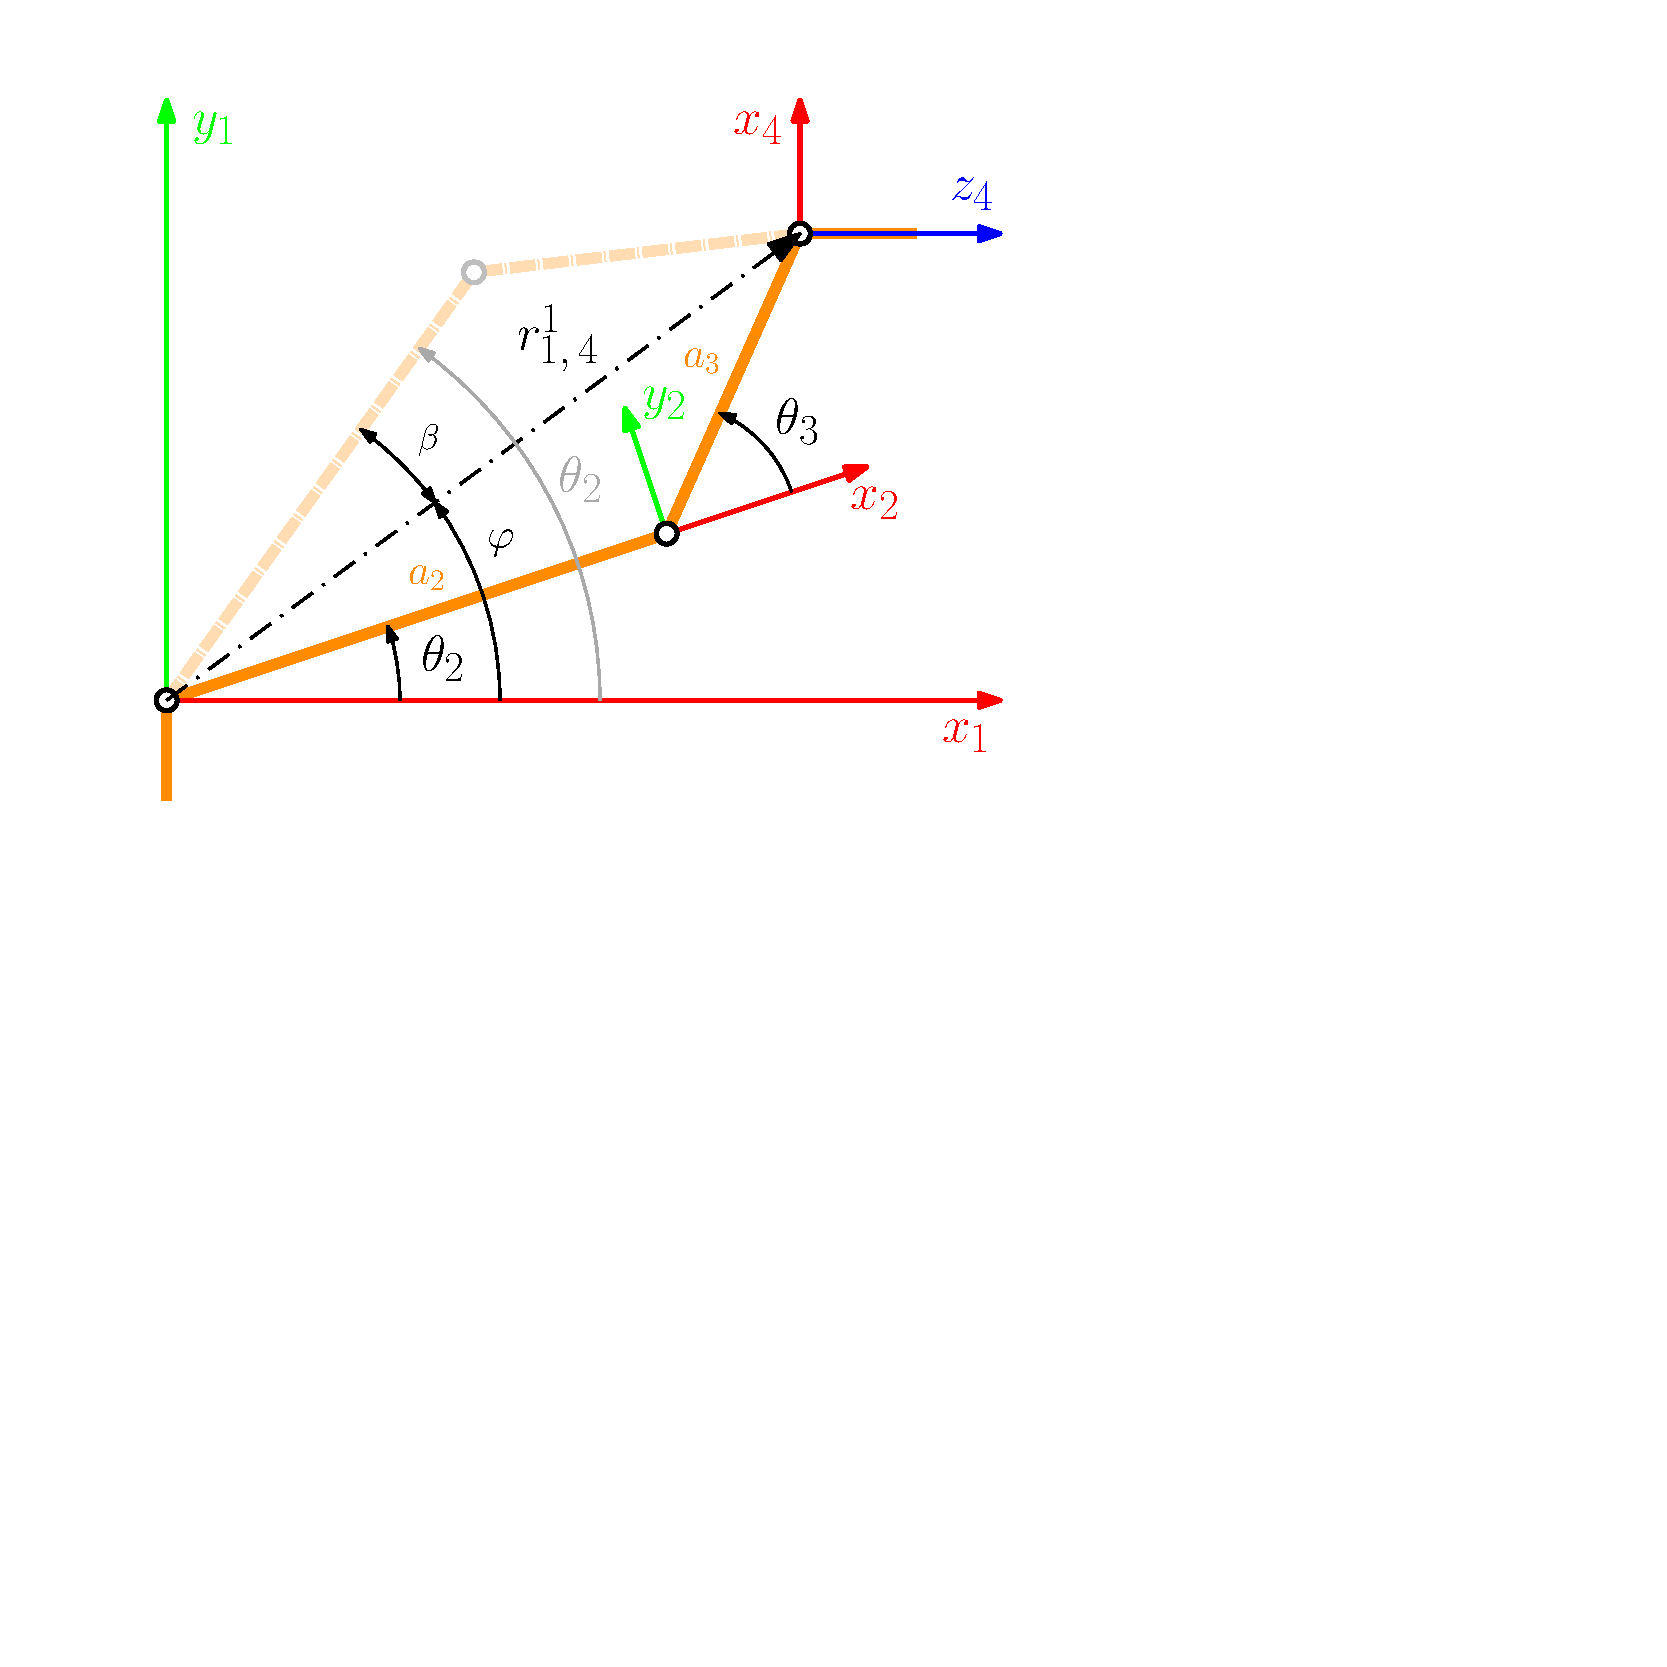
\includegraphics[width=0.7\textwidth]{ik_geometric_approach.pdf}
	\caption{Плоская часть манипулятора}
	\label{ik_geometric}
\end{figure}

Выпишем, пользуясь теоремой косинусов, выражение для $\cos\theta_3$ (его зависимость от $\theta_1$ обуславливается зависимостью от этого угла вектора $r^1_{1,\,4}$):
\begin{equation}
	c_3(\theta_1) = \frac{(r^1_{1,\,4})^T \!\! \cdot r^1_{1,\,4}- a_2^2 - a_3^2}{2 a_2 a_3}
\end{equation}
C~учетом этого для $\theta_3$ можно получить следующие формулы
\begin{gather}
	\theta_3^\msf{I,II} = \mp \atan2\bigl(\sqrt{1 - c_3^2(\theta_1^\msf{I})},\; c_3(\theta_1^\msf{I})\bigr)\\
	\theta_3^\msf{III,IV} = \mp \atan2\bigl(\sqrt{1 - c_3^2(\theta_1^\msf{II})},\; c_3(\theta_1^\msf{II})\bigr)
\end{gather}

Как видно из рисунка~\ref{ik_geometric}, $\theta_2 = \varphi + \beta$ при $\theta_3^\msf{I,III} < 0$ и $\theta_2 = \varphi - \beta$ при $\theta_3^\msf{II,IV} > 0$.
Следовательно, принимая во внимание то, что
\begin{equation}
    \varphi(\theta_1) = \atan2(y_r,\, x_r),
    \qquad
    \beta(\theta_3) = \atan2(a_3\sin|\theta_3|,\: a_2 + a_3\cos|\theta_3|),
\end{equation}
где $x_r$ и $y_r$~--- проекции вектора $r^1_{1,\,4}$ на оси абсцисс и ординат (их значения см.~в~\eqref{eq_r_1_1_4}), для возможных значений угла $\theta_2$ получаем следующие формулы:
\begin{align}
	\theta_2^\msf{I} &= \varphi(\theta_1^\msf{I}) + \beta(\theta_3^\msf{I}), &
	\theta_2^\msf{II} &= \varphi(\theta_1^\msf{I}) - \beta(\theta_3^\msf{II}),\\
	\theta_2^\msf{III} &= \varphi(\theta_1^\msf{II}) + \beta(\theta_3^\msf{III}), &
	\theta_2^\msf{IV} &= \varphi(\theta_1^\msf{II}) - \beta(\theta_3^\msf{IV})\ldotp
\end{align}

Формулы для значений угла $\theta_4$ после этого с учетом~\eqref{eq_theta_23_234} приобретают простой вид:
\begin{equation}
	\theta_4^\msf{I,II} = \theta_{234}^\msf{I} - \theta_{2}^\msf{I,II} - \theta_{3}^\msf{I,II},
	\qquad
	\theta_4^\msf{III,IV} = \theta_{234}^\msf{II} - \theta_{2}^\msf{III, IV} - \theta_{3}^\msf{III,IV}\ldotp
\end{equation}

Таким образом, любые положение и ориентацию схвата относительно основания манипулятор может обеспечить 4-мя собственными конфигурациями, которым соответствуют следующие наборы значений для его обобщенных координат $q=\left[q_1,\,q_2,\,q_3,\,q_4,\,q_5\right]$ (с~учетом таблицы~\ref{table_DH_params}):
\begin{align}
	q^\msf{I} &=
	\begin{bmatrix}
	    \theta_1^\msf{I} & \theta_2^\msf{I} - \cfrac{\pi}{2} & \theta_3^\msf{I} & \theta_4^\msf{I} & \theta_5^\msf{I}
	\end{bmatrix}\!\!,
	&
	q^\msf{II} &=
	\begin{bmatrix}
	    \theta_1^\msf{I} & \theta_2^\msf{II} - \cfrac{\pi}{2} & \theta_3^\msf{II} & \theta_4^\msf{II} & \theta_5^\msf{I}
	\end{bmatrix}\!\!,
	\\
	q^\msf{III} &=
	\begin{bmatrix}
	    \theta_1^\msf{II} & \theta_2^\msf{III} - \cfrac{\pi}{2} & \theta_3^\msf{III} & \theta_4^\msf{III} & \theta_5^\msf{II}
	\end{bmatrix}\!\!,
	&
	q^\msf{IV} &=
	\begin{bmatrix}
	    \theta_1^\msf{II} & \theta_2^\msf{IV} - \cfrac{\pi}{2} & \theta_3^\msf{IV} & \theta_4^\msf{IV} & \theta_5^\msf{II}
	\end{bmatrix}\!\!\ldotp
\end{align}

\newpage